%%%%%%%%%%%%%%%%%%%%%%%%%%%%%%%%%%%%%%%%%%%%%%%%%%%%%%%%%%%%%%%%%%%%%%%%%%%%%%%%%%%%%%
% Modelo de relatório de Disciplina de MLP a partir da
% classe latex iiufrgs disponivel em http://github.com/schnorr/iiufrgs
%%%%%%%%%%%%%%%%%%%%%%%%%%%%%%%%%%%%%%%%%%%%%%%%%%%%%%%%%%%%%%%%%%%%%%%%%%%%%%%%%%%%%%

%%%%%%%%%%%%%%%%%%%%%%%%%%%%%%%%%%%%%%%%%%%%%%%%%%%%%%%%%%%%%%%%%%%%%%%%%%%%%%%%%%%%%%
% Definição do tipo / classe de documento e estilo usado
%%%%%%%%%%%%%%%%%%%%%%%%%%%%%%%%%%%%%%%%%%%%%%%%%%%%%%%%%%%%%%%%%%%%%%%%%%%%%%%%%%%%%%
%
\documentclass[rel_mlp]{iiufrgs}

%%%%%%%%%%%%%%%%%%%%%%%%%%%%%%%%%%%%%%%%%%%%%%%%%%%%%%%%%%%%%%%%%%%%%%%%%%%%%%%%%%%%%%
% Importação de pacotes
%%%%%%%%%%%%%%%%%%%%%%%%%%%%%%%%%%%%%%%%%%%%%%%%%%%%%%%%%%%%%%%%%%%%%%%%%%%%%%%%%%%%%%
% (a A seguir podem ser importados os pacotes necessários para o documento, de acordo 
% com a necessidade)
%
\usepackage{float}
\usepackage[brazilian]{babel}	    % para texto escrito em pt-br
\usepackage[utf8]{inputenc}         % pacote para acentuação
\usepackage{graphicx}         	    % pacote para importar figuras
\usepackage[T1]{fontenc}            % pacote para conj. de caracteres correto
\usepackage{times}                  % pacote para usar fonte Adobe Times
\usepackage{enumerate}              % para lista de itens com letras
\usepackage{breakcites}
\usepackage{titlesec}
\usepackage{enumitem}
\usepackage{titletoc}               
\usepackage{listings}			    % para listagens de código-fonte
\usepackage{mathptmx}               % p/ usar fonte Adobe Times nas formulas matematicas
\usepackage{url}                    % para formatar URLs
%\usepackage{color}				    % para imagens e outras coisas coloridas
%\usepackage{fixltx2e}              % para subscript
%\usepackage{amsmath}               % para \epsilon e matemática
%\usepackage{amsfonts}
%\usepackage{setspace}			    % para mudar espaçamento dos parágrafos
%\usepackage[table,xcdraw]{xcolor}  % para tabelas coloridas
%\usepackage{longtable}             % para tabelas compridas (mais de uma página)
%\usepackage{float}
%\usepackage{booktabs}
%\usepackage{tabularx}
%\usepackage[breaklinks]{hyperref}

\usepackage[alf,abnt-emphasize=bf]{abntex2cite}	% pacote para usar citações abnt

%%%%%%%%%%%%%%%%%%%%%%%%%%%%%%%%%%%%%%%%%%%%%%%%%%%%%%%%%%%%%%%%%%%%%%%%%%%%%%%%%%%%%%
% Macros, ajustes e definições
%%%%%%%%%%%%%%%%%%%%%%%%%%%%%%%%%%%%%%%%%%%%%%%%%%%%%%%%%%%%%%%%%%%%%%%%%%%%%%%%%%%%%%
%

% define estilo de parágrafo para citação longa direta:
\newenvironment{citacao}{
    %\singlespacing
    %\footnotesize
    \small
    \begin{list}{}{
        \setlength{\leftmargin}{4.0cm}
        \setstretch{1}
        \setlength{\topsep}{1.2cm}
        \setlength{\listparindent}{\parindent}
    }
    \item[]}{\end{list}
}

% adiciona a fonte em figuras e tabelas
\newcommand{\fonte}[1]{\\Fonte: {#1}}

% Ative o seguinte caso alguma nota de rodapé fique muito longa e quebre entre múltiplas
% páginas
%\interfootnotelinepenalty=10000

%%%%%%%%%%%%%%%%%%%%%%%%%%%%%%%%%%%%%%%%%%%%%%%%%%%%%%%%%%%%%%%%%%%%%%%%%%%%%%%%%%%%%%
% Informações gerais                                   
%%%%%%%%%%%%%%%%%%%%%%%%%%%%%%%%%%%%%%%%%%%%%%%%%%%%%%%%%%%%%%%%%%%%%%%%%%%%%%%%%%%%%%

% título
\title{Grupo Equipe 7 \\ Projeto Space Invaders Utilizando Lua} 

% autor
\author{Fischer Comerlato}{Felipe} % {sobrenome}{nome}
\author{Eich}{Leonardo} % {sobrenome}{nome} 

% Professor orientador da disciplina
\advisor[Prof.~Dr.]{Mello Schnorr}{Lucas}

% Nome do(s) curso(s):
\course{Curso de Graduação em Ciência da Computa{\c{c}}{\~a}o e Engenharia de Computação}

% local da realização do trabalho 
\location{Porto Alegre}{RS} 

% data da entrega do trabalho (mês e ano)
\date{09}{2018}


% Palavras chave
\keyword{Palavra-chave1}
\keyword{Palavra-chave2}
\keyword{Palavra-chave3}


%%%%%%%%%%%%%%%%%%%%%%%%%%%%%%%%%%%%%%%%%%%%%%%%%%%%%%%%%%%%%%%%%%%%%%%%%%%%%%%%%%%%%%
% Início do documento e elementos pré-textuais
%%%%%%%%%%%%%%%%%%%%%%%%%%%%%%%%%%%%%%%%%%%%%%%%%%%%%%%%%%%%%%%%%%%%%%%%%%%%%%%%%%%%%%

% Declara início do documento
\begin{document}

% inclui folha de rosto 
\maketitle      

\selectlanguage{brazilian}

% Sumario
\tableofcontents



%%%%%%%%%%%%%%%%%%%%%%%%%%%%%%%%%%%%%%%%%%%%%%%%%%%%%%%%%%%%%%%%%%%%%%%%%%%%%%%%%%%%%
% Aqui comeca o texto propriamente dito
%%%%%%%%%%%%%%%%%%%%%%%%%%%%%%%%%%%%%%%%%%%%%%%%%%%%%%%%%%%%%%%%%%%%%%%%%%%%%%%%%%%%%

%espaçamento entre parágrafos
%\setlength{\parskip}{6 pt}

\selectlanguage{brazilian}



%%%%%%%%%%%%%%%%%%%%%%%%%%%%%%%%%%%%%%%%%%%%%%%%%%%%%%%%%%%%%%%%%%%%%%%%%%%%%%%%%%%%%
% Introdução
%
\chapter{Introdução} \label{intro}

Este trabalho tem como objetivo o estudo de uma linguagem de programação moderna com características híbridas contextualizando os conceitos vistos em aula ao longo do semestre e, por fim, analisar e avaliar diferentes linguagens de programação, seguindo os critérios vistos em aula.

A tarefa principal do trabalho consiste em experimentar e comparar as características e funcionalidades orientadas a objeto e funcionais da linguagem de programação escolhida. De posse de uma linguagem, é necessário escolher um problema a ser solucionado com ela. O problema será, então, implementado duas vezes na mesma linguagem: uma delas usando somente Orientação a Objetos e a outra usando somente características funcionais.

O desenvolvimento do trabalho encontra-se em \url{https://github.com/felipefcomerlato/mlp_equipe7_2018-2}.


\section{O Problema}
O problema a ser resolvido neste trabalho é o desenvolvimento do jogo Space Invaders. O jogo expõe o jogador como uma espaçonave que deve destruir as espaçonaves inimigas que querem invadir o planeta do jogador. Na medida que elas avançam na tela (de cima para baixo), o jogador guia sua espaçonave horizontalmente e efetua disparos para destruir todas as ondas de inimigos que se seguem, como visto na figura \ref{fig:figura1}


\begin{figure}[H]
     \centering
     \caption{Tela do jogo Space Invaders}
     \fbox{
         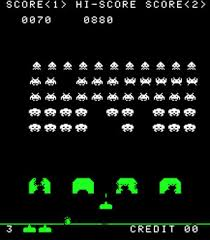
\includegraphics[width=5cm, keepaspectratio]{images/space-invaders-screen.jpeg}
     }
     \label{fig:figura1}
 \end{figure}


\chapter{Visão Geral da Linguagem}

A linguagem escolhida para o trabalho foi \textbf{Lua}. Esta é uma linguagem de alto nível, leve, poderosa e multiparadigma: pode ser considerada de \textit{scripting}, imperativa, funcional ou orientada a objetos. Um dos pontos fortes da linguagem é sua semântica extensível, à qual podem ser adicionadas novas funcionalidades sem alterar suas características originais. Uma das características principais da linguagem é sua única estrutura de dados: tabelas - que podem ser usadas para representar arrays comuns, sequências, tabelas de símbolos, conjuntos, registros, grafos, árvores, etc.

\section{Modelo Funcional}

Lua oferece suporte ao modelo de programação funcional mas nos proporciona algumas dificuldades, como a de copiar tabelas, por exemplo, já que tal estrutura de dados atribuída a uma variável é apenas uma referência. Tal dificuldade contraria uma das principais características do próprio paradigma funcional: a de usar funções puras, criando novas estruturas ao invés de alterar uma estrutura original. Por outro lado, Lua nos permite representar funções anônimas através de blocos de código chamados de \textit{trechos}, característico no modelo funcional.

\section{Modelo Orientado a Objetos}

O suporte para a programação no paradigma orientado a objetos utilizando Lua é muito vasto. É possível encontrar inúmeros tutoriais para a solução de diversos problemas na linguagem fazendo uso deste paradigma. Como não vimos diversos pré-requisitos necessários para a implementação deste trabalho, não podemos analisar com mais propriedade o desempenho da linguagem Lua neste modelo de programação.


% ----------------------- %

\chapter{Recursos Funcionais}

\section{Elementos Imutáveis e Funções Puras}

\section{Funções Anônimas}

\section{Currying}

\section{Pattern Matching}

\section{Funções de Ordem Superior}

\section{Funções de Ordem Maior Fornecidas Pela Linguagem}

\section{Funções como Elementos de Primeira Ordem}

\section{Recursão}

% ----------------------- %

\chapter{Recursos de Orientação à Objetos}

\section{Classes}

\section{Encapsulamento e Proteção dos Atributos}

\section{Construtores}

\section{Destrutores}

\section{Espaços de Nomes Diferenciados}

\section{Mecanismos de Herança}

\section{Polimorfismo por Inclusão}

\section{Polimorfismo Paramétrico}

\section{Polimorfismo por Sobrecarga}

\section{Delegates}

\chapter{Conclusão Final}




% ------ DAQUI PRA BAIXO É SÓ DO MODELO DADO PELO PROF -------------- %

\subsection{Sobre o Sumário}

Relaciona as principais divisões e seções do texto, na mesma ordem em que nele se sucedem, indicando, ainda, as respectivas páginas iniciais. O sumário deverá ser localizado imediatamente após as folhas de rosto, catalogação na publicação, dedicatórias e agradecimentos. Para maiores detalhes, ver a norma NBR-6027 da ABNT (1989b). 

%\paragrafo

Os títulos das subdivisões do texto são apresentados em fonte tamanho 12 pt, com as seguintes variações de estilo: 

\begin{itemize}[leftmargin=3em] % [label={--}]

\setlength{\itemindent}{1em}

    \item \textbf{Capítulos}: fonte Helvetica, negrito, todas em maiúsculas;

    \item \textbf{Seções}: fonte Times, negrito;

    \item \textbf{Subseções}: fonte Times, normal. 

\end{itemize}

Não devem ser incluídos títulos das seções de 4o. e 5o. nível, nem o detalhamento dos Apêndices e/ou Anexos. 

O documento atual já utiliza estilos e comandos \LaTeX\ apropriados para a construção correta do sumário. 

No caso de o trabalho ser apresentado em mais de um volume, cada um deve conter o sumário geral da obra, bem como seu próprio sumário, ocupando páginas consecutivas. 



\subsubsection{sobre a Lista de Abreviaturas e Siglas}

Todas as abreviaturas e siglas devem ser ordenadas alfabeticamente e seguidas de seus respectivos significados. Um exemplo pode ser visualizado no início deste documento. 



\subsubsection{Sobre a Lista de Símbolos}

Semelhante à lista de abreviaturas e siglas, os símbolos utilizados no documento devem ser apresentados na ordem em que nele aparecem, acompanhados de seus respectivos significados. 



\subsubsection{Sobre as Listas de Figuras e de Tabelas}

Separadamente para as Figuras e Tabelas, devem ser relacionadas as ilustrações na ordem em que aparecem no texto, indicando, para cada uma, o seu número, legenda e página onde se encontra.

O documento atual já utiliza estilos e comandos \LaTeX\ apropriados para a construção correta das listas de Figuras e Tabelas. 



\subsection{Numeração das Páginas}

Os números de página são colocados na margem superior do documento, a 2~cm da borda superior do papel, alinhados à {\it margem externa} do texto. Por margem externa entende-se a margem direita nas páginas ímpares e a esquerda nas páginas pares. Quando o documento é produzido somente-frente, utiliza-se sempre a margem direita para a numeração. 

Todas as páginas do documento, a partir da folha de rosto, são contadas, mas a numeração só é mostrada a partir do primeiro capítulo de texto propriamente dito (ou seja, normalmente a Introdução). Assim, as primeiras páginas não devem apresentar numeração.

O documento atual já utiliza estilos \LaTeX\ apropriados para a inserção correta da numeração de páginas. 



%%%%%%%%%%%%%%%%%%%%%%%%%%%%%%%%%%%%%%%%%%%%%%%%%%%%%%%%%%%%%%%%%%%%%%%%%%%%%%%%%%%%%
% Capítulo 2
%
\chapter{AS ILUSTRAÇÕES NO TEXTO}

As ilustrações no texto são geralmente apresentadas ou como Figuras ou como Tabelas. Devem ser acompanhadas de uma legenda explicativa, na qual devem constar o tipo de ilustração (texto "Figura" ou "Tabela"), o respectivo número de ordem, e o texto que descreve a ilustração. Os números de ordem são subordinados ao capítulo onde aparecem, devendo ser apresentados na forma ``X.Y'', onde X é o número do capítulo e Y é o número de ordem da ilustração dentro do capítulo. As numerações de Figuras e Tabelas são independentes entre si. Veja exemplos de legendas nas ilustrações deste documento. 

O documento atual já utiliza estilos \LaTeX\ apropriados para a inserção correta da formatação e numeração de Figuras e Tabelas. 


\section{Descrição das Figuras}

Veja exemplo de formatação da figura \ref{fig:figura1} a seguir: a legenda aparece acima da ilustração, a descrição deve ser centralizada, no número de identificação  \ref{fig:figura1}, o número 2 corresponde ao capítulo onde se localiza a figura e o número 1 a ordem da figura dentro do capítulo, seguido de dois ponto, espaço e a breve descrição da figura, que deve ter a {\bf primeira} letra em maiúsculo.


\begin{figure}[htb]
    \centering
    \caption{Exemplo de apresentação de uma figura no texto}
    \fbox{
        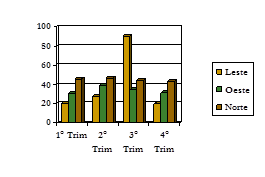
\includegraphics[width=6cm,height=4cm,keepaspectratio]{images/image1.png}
    }
    \label{fig:figura1}
    \fonte{xxxxxx}
\end{figure}


Se  buscada em alguma obra publicada, deve aparecer a fonte da figura, como no exemplo. Caso elaborada pelo próprio autor, incluir "Fonte: autor". Observando que na LISTA DE TABELAS a fonte não deve aparecer. 



\section{Descrição das Tabelas}

Veja exemplo de formatação da Tabela \ref{tab:tabela2}: a legenda aparece acima da tabela, a descrição deve ser centralizada, no número de identificação 2.1, o número 2 corresponde ao capítulo onde se localiza a tabela e o número 1 a ordem da tabela dentro do capítulo, seguido de dois ponto, espaço e  breve descrição, que deve ter a {\bf primeira} letra em maiúsculo. 

Assim como figuras, tabelas também devem indicar sua fonte. Caso elaboradas pelo próprio autor, incluir "Fonte: autor". Observando que na LISTA DE TABELAS a fonte não deve aparecer. 

Atente que {\bf as laterais das tabelas são abertas}. Isso torna a imagem mais limpa e clara. As tabelas do texto não devem exceder a margem.


\begin{table}[ht]
  \caption{Exemplo de apresentação de uma tabela no texto}
  \centering
    \begin{tabular}{ c | c | c }
        \hline 
        \textit{Manga} & 
        \textit{Abacaxi} &  
        \textit{Morango}  \\
        \hline
        12    & 100.000,00     & 10.000,00 \\
        \hline
        12    & 10.000,00     & 100.000,00 \\
      \hline
    \end{tabular}
   \fonte{EREGALI, 2004. p. 356.}
  \label{tab:tabela2}
\end{table}



%%%%%%%%%%%%%%%%%%%%%%%%%%%%%%%%%%%%%%%%%%%%%%%%%%%%%%%%%%%%%%%%%%%%%%%%%%%%%%%%%%%%%
% Capítulo 3
%
\chapter{Sobre referências e citações}

A classe \emph{iiufrgs} faz uso do pacote \emph{abnTeX2} com algumas alterações
feitas por Sandro Rama Fiorini. Culpe ele se algo der errado. Agradeça a ele
pelo que der certo. As modificações dão uma camada de tinta NATBIB-style,
já que o abntex2 usa uns comandos de citação feitos para alienígenas de 5 braços (wtf!?). \\

Exemplos de citação:
\begin{itemize}[leftmargin=3em]

\setlength{\itemindent}{1em}

 \item \textbf{cite}: Unicórnios são verdes \cite{Adams2009Conceptual};
    
 \item \textbf{citet}: Segundo \citet{Adams2009Conceptual}, unicórnios são verdes.
    
 \item \textbf{citeauthoronline e citeyearpar}: Segundo artigos de \citeauthoronline{Adams2009Conceptual}, unicórnios são verdes \citeyearpar{Adams2009Conceptual}.
    
\end{itemize}
 
 
 
Recomenda-se o uso de bibtex para gerenciar as referências (veja o arquivo
biblio.bib).



\section{citações}

Há duas formas de se fazer uma citação: a {\bf indireta} ou {\bf livre} (também chamada de {\it paráfrase}) e a {\bf citação direta} ou {\bf textual}. Pode haver, ainda, a {\bf citação de citação}.

Todas as citações devem trazer a {\bf identificação }de sua autoria.


\section{Citação Indireta ou Livre (paráfrase)}

Chamamos de citação indireta ou livre ({\it paráfrase}) aquela citação na qual expressamos o {\bf pensamento de outra pessoa }com {\bf nossas próprias palavras.}

Após fazermos a citação, devemos indicar o nome do autor, {\bf em letras minúsculas, }se estiver no corpo do texto, e com letras {\bf maiúsculas, }se estiver dentro dos parênteses, juntamente com o {\bf ano }da publicação da obra em que se encontra a idéia por nós referida. Não são indicadas páginas já que a idéia pode estar sendo resumida de uma obra inteira, de um capítulo, de diversas partes ou de um conjunto delas.

Desta forma (com o nome no corpo do texto):

Depois de analisar a situação, Nóvoa (1993) chegou a afirmar que o brasileiro ainda não está capacitado para escolher seus governantes por causa de sua precária vocação política e da absoluta falta de escolaridade, já que o homem do povo, o zé-povinho, geralmente não sabe sequer em quem votou nas últimas eleições, não sabe sequer quem são seus governantes, não saber sequer quem determina seu próprio meio de sobreviver.

Ou, então, (com o nome nos parênteses):

Depois de analisar a situação, chegou-se a afirmar que o brasileiro ainda não está capacitado para escolher seus governantes por causa de sua precária vocação política e da absoluta falta de escolaridade, já que o homem do povo, o zé-povinho, geralmente não sabe sequer em quem votou nas últimas eleições, não sabe sequer quem são seus governantes, não saber sequer quem determina seu próprio meio de sobreviver (NÓVOA, 1993).

No caso de o autor possuir outras obras, elas serão diferenciadas pela data da publicação. Havendo mais de uma obra no mesmo ano, acrescentamos uma letra após a data.

No caso do teatro ou do cinema quem melhor se definiu foi Antunes (1997-a) quando declarou que aqueles espaços haviam sido todos tomados pela geração de 40. Por outro lado, ele próprio se contradisse, mais tarde, (1997-b), como já se contradissera noutras ocasiões, ao referir-se às decisões tomadas pelos autores da geração de 50. Isso é uma incongruência com a qual convivemos há muito tempo.

Quando, no transcorrer do texto, em citações indiretas ou livres, se faz menção, seguidas vezes, ao mesmo autor, na mesma obra, {\bf {\it não é necessário}}{\it  }que{\it  }se repita a indicação do ano.


\begin{table}[ht]
  \caption{Deve-se escolher somente um tipo de citação para usar durante o texto}
  \centering
    \begin{tabular}{ l | p{8cm} }
        \hline
        \multicolumn{2}{c}{FORMATAÇÃO DAS CITAÇÕES DOS AUTORES DURANTE O TEXTO} \\
        \hline
        Nóvoa (1993) & O nome do autor deve ser escrito em letras {\bf minúsculas }quando apresentado no próprio texto \\
        \hline
        (GUIMARÃES, 1985, p.32) & O nome do autor deve ser escrito em letras {\bf maiúsculas }quando apresentado dentro dos parênteses. \\
      \hline
    \end{tabular}
  \\Fonte: MEREGALI, 2004. p. 356.
  \label{tab:tabela3}
\end{table}



\section{Citação Direta ou Textual (transcrição)}

São chamadas de citações diretas ou textuais aquelas em que se transcrevem {\bf exatamente as palavras do autor citado}. As citações diretas ou textuais podem ser {\bf breves }ou {\bf longas.}

São consideradas {\bf breves} aquelas cuja extensão não ultrapassa {\it três linhas. }Essas citações devem {\it integrar o texto e }devem vir {\bf entre aspas. O tamanho }da {\bf fonte }(letra) da citação breve {\bf permanece }o mesmo do corpo do texto {\bf {\it (12 pt).}}

Vimos que, para nosso esclarecimento, precisamos seguir os preceitos encontrados, já que Guimarães estabelece: "A valorização da palavra pela palavra encarna o objetivo precípuo do texto literário" (1985, p. 32) e, se isso não ficar bem esclarecido, nosso trabalho será seriamente prejudicado.

Ou assim:

Vimos que, para nosso esclarecimento, precisamos seguir os preceitos encontrados, já que ficou estabelecido que "a valorização da palavra pela palavra encarna o objetivo precípuo do texto literário" (GUIMARÃES, 1985, p.32) e, se isso não ficar bem esclarecido, nosso trabalho será seriamente prejudicado.

As citações com mais de três linhas são chamadas de {\bf longas }e devem receber um destaque especial{\bf  }com recuo (reentrada) de {\bf 4cm }ou {\bf dezesseis toques}, da margem, mais {\bf cinco }toques para o início do parágrafo, além de usar fonte 10 pt, justificada.

As citações longas, por já terem o destaque do recuo (reentrada), {\bf \underbar{não deverão ter aspas}} e o tamanho da fonte (letra) deve ser {\bf menor }que o do texto: {\bf {\it 10 pt.}}

A distância entre as linhas do corpo da citação deve ser de um espaço {\bf simples}. Entre o texto da citação e o restante do trabalho, deve-se deixar {\bf dois {\it espaços duplos, }}antes e depois.

Há uma certa dificuldade quanto ao reconhecimento de {\bf O}, {\bf A, OS, AS }como pronomes demonstrativos, mas essa dúvida é muito bem dirimida por Fernandes:

\begin{citacao}
Os pronomes O, A, OS e AS passam a ser pronomes demonstrativos sempre que numa frase puderem ser substituídos, sem alterar a estrutura dessa frase, respectivamente, por ISTO, ISSO, AQUILO, AQUELE, AQUELES, AQUELA, AQUELAS (1994, p. 19.).
\end{citacao}


Havendo {\bf supressão }de trechos {\bf dentro do texto }citado, faz-se a indicação com reticências entre colchetes {\bf [...]}: "Na comunicação diária, aquela comunicação que utilizamos no dia-a-dia, junto de nossos familiares e amigos, por exemplo, além da referencialidade da linguagem {\bf [...]} há pinceladas de função conativa" (CHALHUB , 1991, p. 37).

No {\bf início }ou no {\bf fim }da citação, as reticências são usadas apenas quando o trecho citado {\bf não é uma sentença completa}. Entende-se por sentença completa aquela que o autor elaborou, com todos os seus elementos, isto é, uma sentença que contenha sujeito, predicado e seus complementos gramaticais exigidos. Caso contrário, {\bf se a sentença for completa, }no início ou no termino de citação, {\bf não se deve fazer }o uso das reticências. {\bf É {\it óbvio}} que se trata de parte de um todo, que se retirou um trecho, portanto, não há necessidade de se indicar com as reticências.

Encerrava seu discurso nomeando os que figurariam somente nos exercício gerais, citando palavras de ordem, dentre as quais pudemos entender:

``... muitas mortes, desaparecimentos e desolação haverão de varrer este pais de norte a sul, de lesta a oeste e nada restará para a posteridade que sentirá a falta de um elo'' (MORGADO, 1967).

Mais adiante, aquilo que mais chocou a todos quanto o ouviam:

``Arrasem com tudo, queimem tudo, ponham tudo abaixo, destruam com tudo, não poupem ninguém, nem crianças, nem mulheres, nem velhos...'' (MORGADO, 1967).

Se a citação for usada para completar uma{\bf  }sentença do autor do Trabalho, esta terminará em vírgula e aquela iniciará {\bf sem a entrada de parágrafo} e com {\bf letra minúscula}. 

A secretária ameaçou, dizendo que, ``da próxima vez, a máquina ficará sem as peças de reposição, se ele não chegar e disser o que precisa ser dito, uma vez que não estou aqui para servir de adivinha para seus caprichos desencontrados e sem nexo.'' (MARQUES, 1982, p. 34).

Caso o texto do autor do Trabalho seja uma {\bf continuação }da citação, esta {\bf terminará por vírgula }e o texto reiniciado {\bf sem entrada de parágrafo e com letra minúscula.}

 Os gramáticos são claros quando assumem uma posição quanto ao emprego do pronome oblíquo no início de oração. Cegalla (l 991, p. 419) diz claramente que:

\begin{citacao}
 Iniciar a frase com o pronome átono só é lícito na conversação familiar, despreocupada, ou na língua escrita, quando se deseja reproduzir a fala dos personagens, porém nós sabemos que na prática não é bem assim que acontece - as normas, rigorosamente, são esquecidas por quase todos os usuários do idioma falado, principalmente nas ocasiões informais.
\end{citacao}

Quando houver uma citação {\bf {\it dentro de outra citação, }}as aspas da segunda transformam-se em aspas simples ( ' ) (apóstrofo${}^{: }$Não confundir a palavra {\bf {\it apóstrofo}}{\it  que }é o sinal (`), com {\bf {\it apóstrofe}}{\it  que }é uma figura de linguagem que consiste na interpelação ou invocação do leitor, ouvinte ou outra pessoa no decorrer de um texto). Quando dentro da citação transcrita houver aspas, estas também são mudadas para aspas simples.



Se for feita alguma {\bf interpelação, acréscimo }ou {\bf comentário }durante a citação, deve-se fazê-lo {\it entre colchetes }{\bf [ ]:}

Também chamado de corpo do trabalho, [o desenvolvimento] tem por finalidade expor, demonstrar e fundamentar a explicitação do assunto a ser abordado. É normalmente dividido em seções ou capítulos, que variam de acordo com a natureza do assunto. (GARCIA, 2000, p. 17.).

Se algum {\bf destaque }(grifo, negrito, itálico ou sublinhado) for dado, deve-se indicá-lo com a expressão {\bf grifo nosso, }entre colchetes:

A primeira citação de uma obra deve ter sua referência bibliográfica completa. As subseqüentes citações da mesma obra {\bf podem ser referendadas de forma abreviada, }desde que não haja referências intercaladas de outras obras do mesmo autor (NBR 6023-2000) {\bf [grifo nosso].} 

Caso o texto citado traga algum tipo de destaque dado pelo autor do trecho, devemos usar a expressão {\bf grifo do autor, entre colchetes.}

A verdadeira felicidade é encontrada nos pequenos detalhes que vão se somando {\bf dia após dia }de convivência com o ser amado (GUERRERO, 2000, p. 12) {\bf [grifo do autor].}

Quando o texto citado for composto por informações orais obtidas em aulas, palestras, debates, comunicações, etc. deve-se, entre parênteses, colocar a observação {\bf {\it informação oral, }}mencionando-se os dados disponíveis em nota de rodapé:

Eichenberg constatou que, na costa do Rio Grande do Sul, especialmente no litoral norte, há a presença abundante de conformes fecais, especialmente nos meses do verão (informação oral). Essa presença tem causado graves transtornos a todos os veranistas.

Se for o caso de se fazer menção a algo contido em {\it polígrafos, apostilas }ou quaisquer materiais avulsos, faz-se a indicação do nome do autor, quando for possível sua identificação, acrescentando-se a observação {\it `polígrafo', }`{\it material de propaganda', `panfleto', etc. }Procede-se da mesma forma com relação à data. Indica-se, se houver, caso contrário, registra-se s.d. (sem data). 



\section{Citação de Citação}

Se, num Trabalho, for feita uma citação de alguma passagem {\it já}{\bf {\it  }}{\it citada} em {\it outra obra, }a autoria deve ser referenciada pelo {\bf sobrenome do autor original }seguido da palavra latina {\bf apud }(que significa {\it segundo, conforme, de acordo com) }{\bf e o sobrenome do autor da obra consultada. }Dessa última, faz-se a referência completa (NBR6O23).

``O sistema consiste em colocar o recém-nascido no berço, ao lado da mãe, logo após o parto ou algumas horas depois, durante a estada de ambos na maternidade'' (HARUNARI apud GUARAGNA, 1992, p. 79).

Temos aí palavras de Harunari que foram citadas por Guaranga e que estão sendo utilizadas, agora, no meu trabalho.

{\bf Fonte:} FURASTÉ, Pedro Augusto. Normas Técnicas para o Trabalho Científico: explicitação das normas da ABNT. Porto Alegre: [s.n.], 2002. p. 49-56.

\noindent 


%%%%%%%%%%%%%%%%%%%%%%%%%%%%%%%%%%%%%%%%%%%%%%%%%%%%%%%%%%%%%%%%%%%%%%%%%%%%%%%%%%%%%
% Conclusões
%
\chapter{CONCLUSÃO}

Apresentar conclusão do trabalho...




%%%%%%%%%%%%%%%%%%%%%%%%%%%%%%%%%%%%%%%%%%%%%%%%%%%%%%%%%%%%%%%%%%%%%%%%%%%%%%%%%%%
% Referências 
%%%%%%%%%%%%%%%%%%%%%%%%%%%%%%%%%%%%%%%%%%%%%%%%%%%%%%%%%%%%%%%%%%%%%%%%%%%%%%%%%%%
%

%\bibliographystyle{abnt}

\bibliographystyle{abntex2-alf}


\bibliography{biblio} % arquivo que contém as referências (no formato bib). Colocar as suas lá (se tiver dúvida sobre como adicionar novas referências, usar o software JabRef ou Medley)



\noindent {\\\bf Se tiver alguma dúvida, veja os exemplos seguintes:}\\

\noindent {\bf \underbar{Monografia no todo}}\\

\noindent {\bf Livros e Anais de Congresso (Autor. Título. Edição. Local de Publicação: editora, ano de publicação).}\\

\noindent FURASTÉ, Pedro Augusto. {\bf Normas Técnicas para o Trabalho Científico}: explicitação das normas da ABNT. Porto Alegre: [s.n.], 2002. p. 49-56.

\noindent BRADLEY, N. {\bf The XML Companion}. 3${}^{rd}$ ed. Boston: Addison-Wesley, 2002.

\noindent FIELDS, D. K.; KDLB, M. A. {\bf Desenvolvendo na Web com JavaServer Pages}. Rio de Janeiro: Ciência Moderna, 2000.

\noindent OLIVEIRA, R. S. de; CARISSIMI, A. da S.; TOSCANI, S. S. {\bf Sistemas Operacionais}. 2.ed. Porto Alegre: Instituto de Informática da UFRGS: Sagra Luzzatto, 2001. 247 p. (Série Livros Didáticos, n.11).

\noindent SIMPÓSIO BRASILEIRO DE SISTEMAS MULTIMÍDIA E HIPERMÍDIA, SBMÍDIA, 7., 2001, Florianópolis. ... Florianópolis: UFSC: SBC, 2001.

\noindent NATIONAL CONFERENCE ON ARTIFICIAL INTELLIGENCE, AAII, 17., 2000. {\bf Proceedings}... Menlo Park, CA: AAAI Press: The MIT Press, 2000.

\noindent ~

\noindent {\bf \underbar{Parte de Monografia}}\\

\noindent {\bf Capítulo (Autor do capítulo. Título do capítulo. In: Autor/Editor/Organizador do livro. Título do livro. Edição. Local de publicação: editora, ano de publicação).}

\noindent LUBASZEWSKI, M.; COTA, E. F.; KRUG, M. R. Teste e Projeto Visando o Teste de Circuitos e Sistemas Integrados. In: REIS, R. A. da L. (Ed.) {\bf Concepção de Circuitos Integrados}. 2.ed. Porto Alegre: Instituto de Informática da UFRGS: Sagra Luzzatto, 2002. p. 167-189.

\noindent ROESLER, V.; BRUNO, G. G.; LIMA, J. V. de. ALM: Adaptative Layering Multicast. In: SIMPÓSIO BRASILEIRO DE SISTEMAS MULTIMÍDIA, SBMÍDIA, 7., 2001, Florianópolis. {\bf Anais...} Florianópolis: UFSC: SBC, 2001. p. 107-121.

\noindent PFEFFER, A.; KOLLER, D. Semantics and Inference for Recursive Probability Models. In: NATIONAL CONFERENCE ON ARTIFICIAL INTELLIGENCE, AAII, 17., 2000. {\bf Proceedings... }Menlo Park, CA: AAAI Press: The MIT Press, 2000.

\noindent ~

\noindent {\bf \underbar{Dissertações, teses, trabalhos individuais, etc.}}\\

\noindent MENEGHETTI, E. A. {\bf Uma Proposta de Uso da Arquitetura Trace como um Sistema de Detecção de Intrusão}. 2002. 105 f. Dissertação ( Mestrado em Ciência da Computação ) -- Instituto de Informática, UFRGS, Porto Alegre.

\noindent SABADIN, R. da S. {\bf QoS em Serviços de Suporte por Frame Relay}. 2000. 35 f. Trabalho Individual ( Mestrado em Ciência da Computação ) -- Instituto de Informática, UFRGS, Porto Alegre.

\noindent OTERO, I. M. {\bf Desenvolvimento de Sistema Cliente-Servidor em Camadas Utilizando Software Livre}. 2003. 55 f. Projeto de Diplomação ( Bacharelado em Ciência da Computação ) -- Instituto de Informática, UFRGS, Porto Alegre.

\noindent ~

\noindent {\bf \underbar{Artigo de periódico}}\\

\noindent GONÇALVES, L. M. G.; CESAR JUNIOR, R. M. Robótica, Sistemas Sensorial e Motos: principais tendências e direções. {\bf Revista de Informática Teórica e Aplicada}, Porto Alegre, v.9, n.2, p. 7-36, out. 2002.

\noindent JANOWIAK, R. M. Computers and Communications: a symbiotic relationship. {\bf Computer}, New York, v.36, n.1, p. 76-79, Jan. 2003.

\noindent ~

\noindent {\bf \underbar{Em meio eletrônico}}\\

\noindent LISBOA FILHO, J.; IOCHPE, C.; BORGES, K. Reutilização de Esquemas de Bancos de Dados em Aplicações de Gestão Urbana. {\bf IP -- Informática Pública}, Belo Horizonte, v.4, n.1, p.105-119, June 2002. Disponível em: $<$http://www.ip.pbh.gov.br/ip0401.html $>$. Acesso em: set. 2002.

\noindent ~

\noindent {\bf \underbar{RFC}}\\

\noindent CALLAGHAN, B.; PAWLOWSKI, B.; STAUBACH, P. {\bf NFS Version 3 Protocol Specification}: RFC 1831. [S.l.]: Internet Engineering Task Force, Network Working Group, 1995.

\noindent ~

\noindent {\bf \underbar{Norma}}\\

\noindent INSTITUTE OF ELECTRICAL AND ELECTRONIC ENGINEERING. {\bf IEEE 1003.1c-1995}: information technology -- portable operating system interface (POSIX), threads extension [C language]. New York, 1995.

\noindent ~

\noindent {\bf \underbar{Observações}}\\

Quando existirem mais de três autores, indica-se apenas o primeiro, acrescentando-se a expressão et al. Ex.: URANI, A. et al. Em casos em que a menção dos nomes for indispensável para certificar a autoria é facultado indicar todos os nomes.

Em caso de autoria desconhecida, a entrada é feita pelo título. Ex.: DIAGNÓSTICO do Setor Editorial Brasileiro. São Paulo: Câmara Brasileira do Livro, 1993.

Quando houver uma indicação de edição, esta deve ser transcrita, utilizando-se abreviaturas dos numerais ordinais e da palavra edição, ambas na forma adotada na língua do documento.

Ex.: SCHAM, D. {\bf Schawm's Outline of Theory and Problems}. 5${}^{th}$ ed. New York: Schawm Publishing, 1956.

PEDROSA, I. {\bf Da Cor a Cor Inexistente}. 6. ed. Rio de Janeiro: L. Cristiano, 1995.

Não sendo possível determinar o local (cidade) de publicação, utiliza-se à expressão sine loco, abreviada, entre colchetes [S.l.].

Quando a editora não puder ser indicada, deve-se indicar a expressão sine nomine, abreviada, entre colchetes [s.n].

Quando o local e a editora não puderem ser identificados, utilizam-se [S.l.:s.n].




\end{document}
